\documentclass[10pt,a4paper]{article}
\usepackage[utf8]{inputenc}
\usepackage[english]{babel}
\usepackage{amsmath}
\usepackage{amsfonts}
\usepackage{amssymb}
\usepackage{soul}
\usepackage[margin=1in]{geometry}
\usepackage{enumitem}
\usepackage{adjustbox}
\usepackage{multicol}
\usepackage{cancel}
\usepackage{graphicx}

\newlength{\drop}

\usepackage{tikz}

\newcommand{\inline}[2]{%
    \begin{tikzpicture}[baseline=(word.base), txt/.style={shape=rectangle, inner sep=0pt}]% the baseline key ensures that nodes won't shift up if there's text with descenders, and the txt style removes extra spacing so you can use this inline
    \node[txt] (word) {#1};% the first argument is the contents of the main node
    \node[above] at (word.north) {\footnotesize{#2}};% the second argument is the tag; you can play with the positioning as necessary
    \end{tikzpicture}%
    }

\begin{document}

\begin{titlepage}

\drop=0.1\textheight
    \centering
    \vspace*{\baselineskip}
    \rule{\textwidth}{1.6pt}\vspace*{-\baselineskip}\vspace*{2pt}
    \rule{\textwidth}{0.6pt}\\[\baselineskip]
    {\LARGE APUNTES DE\\[0.2\baselineskip] ROBOTICA}\\[0.2\baselineskip]
    \rule{\textwidth}{0.4pt}\vspace*{-\baselineskip}\vspace{3.2pt}
    \rule{\textwidth}{1.6pt}\\[\baselineskip]
    \scshape
    MODELO CINEMÁTICO DE VELOCIDAD \\
    \vspace*{2\baselineskip}
    %Edited by \\[\baselineskip]
    %{\Large MAXIMILIANO PONCE\par}
    %{\itshape My notes from \\Langpill english grammar course from Udemy, and Grammarly\\\par}
    \vfill
    {\scshape Abril 2020} \\
    {\large MAXIMILIANO PONCE}\par

\end{titlepage}

\tableofcontents
\newpage

\section{Modelo cinemático de velocidad}
En esta sección se derivan las relaciones de velocidad, con respecto a las velocidades lineales y angulares del efector final. Las relaciones de velocidad se determinan por los Jacobianos de la cinemática directa.\\

\section{Velocidad angular: Caso de eje fijo}

\begin{figure}[h]
     \centering
     \begin{center}
		 $\omega = \dot{\theta} \vec{k}$ \\
     	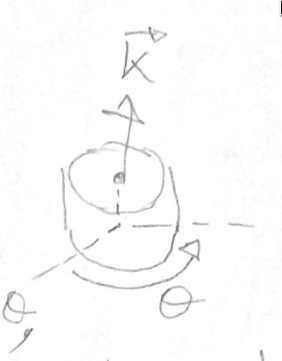
\includegraphics[width=0.2\linewidth]{f1}
     \end{center}
\end{figure}


donde $\dot{\theta}$ es la derivada con respecto al tiempo de $\theta$, $\vec{k}$ es un vector en dirección del eje de rotación y $\omega$ es la velocidad angular. Dada la velocidad angular del cuerpo, la velocidad lineal de cualquier punto en el cuerpo esta dada por:

$$ \upsilon = \omega \times \vec{r}$$

donde $\vec{r}$ es un vector desde el origen al punto dado. La velocidad angular $\omega$ es una propiedad de la trama anexa al cuerpo. La velocidad angular no es una propiedad de un punto particular. Asi que $\upsilon$ corresponde a la velocidad lineal de un punto mientras $\omega$ corresponde a la velocidad angular de una trama rotando.

\section{Matrices asimétricas}
Se dice que una matriz $S$ es asimétrica si y sólo si:
$$ S^T + S = 0$$

donde,
$$
	S =
	\begin{bmatrix}
		0    & -s_3 & s_2\\
		s_3  & 0    & -s_1\\
		-s_2 & s_1  & 0
	\end{bmatrix}
$$

\textbf{Por ejemplo}: si se definen a los tres vectores unitarios de un sistema de coordenadas como $\vec{i}$, $\vec{j}$, $\vec{k}$, representados como:
$$
	\vec{i} =
	\begin{bmatrix}
		1 \\ 0 \\ 0
	\end{bmatrix},
	\vec{j} =
	\begin{bmatrix}
		0 \\ 1 \\ 0
	\end{bmatrix},
	\vec{k} =
	\begin{bmatrix}
		0 \\ 0 \\ 1
	\end{bmatrix}
$$

Entonces las matrices asimétricas $S(\vec{i}), S(\vec{j}), S(\vec{k})$ se definen como:

$$
	S(\vec{i}) =
	\begin{bmatrix}
		0 & 0 & 0 \\
		0 & 0 & -1\\
		0 & 1 & 0
	\end{bmatrix},
	S(\vec{j}) =
	\begin{bmatrix}
		0 & 0 & 1 \\
		0 & 0 & 0\\
		-1& 0 & 0
	\end{bmatrix},
	S(\vec{k}) =
	\begin{bmatrix}
		0 & -1 & 0 \\
		1 & 0 & 0\\
		0 & 0 & 0
	\end{bmatrix}
$$

Derivada de una matriz de rotación:

$$
	R(\theta) \cdot R(\theta)^T=I
$$

Obteniendo la derivada de la ecuación anterior se tiene:


$$
	\frac{dR}{d\theta} \cdot R(\theta)^T + R(\theta) \cdot \frac{dR^T}{d\theta} = 0
$$

\begin{multicols}{2}

	Se define a $S$ como,

	$$ S:=\frac{dR}{d\theta} \cdot R(\theta)^T $$

	entonces, la transpuesta de $S$ es,

	$$ S^T = \left( \frac{dR}{d\theta} \cdot R(\theta)^T \right)^T = R(\theta) \cdot \frac{dR^T}{d\theta} $$

	Por lo que se cumple

	$$ S + S^T = 0$$

	\columnbreak
	\fbox{\begin{minipage}{15em}
	\textbf{Demostración} \\
	$$ S = \frac{dR}{d\theta} \cdot R(\theta)^T $$
	$$ \frac{dR}{d\theta} = \frac{S}{R(\theta)^T} $$
	$$ R(\theta)^T = R(\theta)^{-1} = \frac{1}{R(\theta)} $$
	$$ \frac{dR}{d\theta} = \frac{S}{ \frac{1}{R(\theta)} } $$
	$$ \frac{dR}{d\theta} = S \cdot R(\theta) $$
	\end{minipage}}
\end{multicols}

En otras palabras la matriz $S$ es una matriz asimétrica. Entonces,

$$ S \cdot R(\theta) = \frac{dR}{d\theta} R(\theta) R(\theta)^T $$

\[
	\boxed{\frac{dR}{d\theta} = S R(\theta)} \quad \dot{R}(\theta) = S R(\theta)
 \]

\vspace{0.5cm}

 \textbf{Ejemplo:} Si $R=R_{\vec{x},\theta}$ donde  $R_{\vec{x}}$ se refiere a la matriz de rotación básica que se gira sobre el eje $x$, entonces

 $$
	S = \frac{dR}{d\theta} R^T = \frac{d}{d\theta}
	\begin{Bmatrix}
	\begin{bmatrix}
		1 & 0 & 0 \\
		0 & c\theta & -s\theta\\
		0 & s\theta & c\theta
	 \end{bmatrix}
	 \end{Bmatrix}
	\cdot
	 \begin{bmatrix}
	 	1 & 0 & 0 \\
		0 & c\theta & -s\theta\\
		0 & s\theta & c\theta
	 \end{bmatrix}^T =
	\begin{bmatrix}
	 	0 & 0 & 0 \\
		0 & -s\theta & -c\theta\\
		0 & c\theta & -s\theta
	 \end{bmatrix} \cdot
	 \begin{bmatrix}
	 	1 & 0 & 0 \\
		0 & c\theta & s\theta\\
		0 & -s\theta & c\theta
	 \end{bmatrix}
 $$

 $$
	S =
	\begin{bmatrix}
		0 & 0 & 0 \\
		0 & \cancel{-s\theta c\theta + s\theta c\theta} & -s^2\theta - c^2\theta \\
		0 & c^2\theta + s^2\theta & \cancel{s\theta c\theta - s\theta c\theta}
	\end{bmatrix} =
	\begin{bmatrix}
		0 & 0 & 0 \\
		0 & 0 & -1 \\
		0 & 1 & 0
	\end{bmatrix} = S(i)
 $$
\vspace{0.5cm}
\section{Velocidad angular: Caso general}

 Suponiendo que $R(t)$ varia con el tiempo,

 $$ \dot{R}(t) = S(t)R(t)	$$

 Como $S(t)$ es asimétrica puede representarse como $S(\omega(t))$ para un vector único $\omega(t)$. El vector $\omega(t)$ es la velocidad angular de una trama de rotación con respecto a una trama fija en un tiempo $t$.

 $$ \dot{R}(t) = S(\omega(t))R(t) $$

 Cuando la trama fija es $O_0$ con respecto a una trama movil $O_n$,

 $$ \dot{R}_{n}^{0} = S(\omega_{o,n}^0)R_n^0 $$

 Velocidad lineal de un un punto fijo a una trama movil. Las coordenadas de $p^1$ con respecto a la trama $O_0$ estan dados por:

 $$ p^0 = R_1^0 p^1$$

 La velocidad $\dot{p}^0$ esta dado por

 $$ \dot{p}^0 = \dot{R}_1^0(t) p^1 + R_1^0(t) \cancel{\dot{p}^1} $$

 debido a que $p^1$ se encuentra fijo a la trama $O_1$ y las coordenadas relativas a la trama $O_1$ no cambian entonces

 $$ \dot{p}^1 = 0 \quad \dot{p}^0 = \dot{R}_1^0(t) p^1 = S(\omega^0)R_1^0 p^1 = S(\omega^0) p^0 $$

 $$ \dot{p}^0 = \omega^0 \times p^0 $$

 Suponiendo que la transformación homogenea es dependiente del tiempo, entonces:

 $$
	H_1^0 =
	\begin{bmatrix}
		R_1^0(t) & O_1^0(t) \\
		O & 1
	\end{bmatrix}
 $$

 Si se omite por simplicidad el argumento $t$ y también superíndices y los subíndices en $R_1^0$ y $O_1^0$ se escribe,

 $$ p^0 = R p^1 + O $$

 Si se diferencia la expresión anterior,

 $$ \dot{p}^0 = \dot{R} p^1 + \dot{O}$$
 $$ \dot{p}^0 = S(\omega) R_{p^1} + \dot{O}$$
 $$ \dot{p}^0 = \omega \times r + \upsilon$$

 donde $r=R_{p^1}$ es el vector dese $O_1$ a $p$ que se expresa en la orientación de la trama $O_0$ y $\upsilon$ es la tasa a la cual el origen $O_1$ se mueve.

\section{Derivación del Jacobiano}
Considere un manipulador de n-eslabones y con variables de articulación $q_1 \dots, q_n$ tal que:

$$
	T_n^o(q) =
	\begin{bmatrix}
		R_n^o(q) & O_n^o(q) \\
		O_n & 1
	\end{bmatrix}
$$

El objetivo de esta sección es relacionar la velocidad lineal y angular del efector-final con el vector de velocidades de articulación $\dot{q}(t)$. Se defina la velocidad $\omega_n^o$ del efector-final:

$$ S(\omega_n^o) = \dot{R}_n^o (R_n^0)^T $$

y la velocidad lineal del efector-final como,

$$ \upsilon_n^o = \dot{O}_n^o $$

Se desean expresiones de la forma:

$$ \upsilon_n^o = J_{\upsilon} \dot{q} $$
$$ \omega_n^o = J_{\omega} \dot{q} $$

donde $J_{\upsilon}$ y $J_{\omega}$ son matrices $3 \times n$. Agrupando se tendrá,

$$ \epsilon = J \dot{q} $$

donde $\epsilon$ y $J$ estan dados por:

$$ \epsilon =
\begin{bmatrix}
	\upsilon_n^o\\
	\omega_n^o
\end{bmatrix},
J =
\begin{bmatrix}
	J_{\upsilon}\\
	J_{\omega}
\end{bmatrix}
$$

$\epsilon$ es llamada velocidad del cuerpo y $J$ Jacobiano. La matriz $J$ es una matriz de $ 6 \times n$ donde $n$ es el número de articulaciones.

\section{Velocidad angular}

Si la i-ésima articulación es revoluta, entonces la i-ésima variable de articulación $q_i$ se iguala como $\theta_i$ y el eje de rotación es $\vec{z}_{i-1}$. Se propone a $\omega_i^{i-1}$ como la velocidad angular del eslabón $i$ que se propaga por la rotación de la articulación $i$ expresado relativo a la trama $O_{i-1} x_{i-1} y_{i-1}  z_{i-1}$ (trama anterior).

La velocidad angular se expresa en la trama $i-1$ por,

$$ \omega_i^{i-1} = \dot{q}_i \vec{z}_{i-1}^{i-1} = \dot{q}_i \vec{k} $$

donde $\vec{k}$ es el vector de coordenadas unitarias
$ \begin{bmatrix}
	0 & 0 & 1
\end{bmatrix}^T$. \\
Si la i-ésima articulación es prismática, entonces $i-1$ es una transportación y,

$$ \omega_i^{i-1} = O $$

En este caso $\dot{q}_i \neq d_i$. La velocidad angular total del efector-final esta dada por:

$$ \omega_n^o = \rho_1 \dot{q}_1 \vec{k} + \rho_2 \dot{q}_2 R_1^o \vec{k} + \cdots + \rho_n \dot{q}_n R_{n-1}^o \vec{k} = \sum_{i-1}^{n} \rho_n \dot{q}_i z_{i-1}^o$$

en donde $\rho_1 = 1$ si la articulación $i$ es revoluta y $\rho_1 = 0$ si es prismática. También $z_{i-1}^o = R_{i-1}^o \vec{k}$

\begin{multicols}{2}

	$$ z_o^o = \vec{k} = \begin{bmatrix}
		0 & 0 & 1
	\end{bmatrix}^T $$

	Entonces $J$ Jacobiano de velocidad angular esta dado por:

	$$ J_\omega = \begin{bmatrix}
		\rho_1 z_o \cdots \rho_n z_{n-1}
	\end{bmatrix} $$

	\columnbreak
	\fbox{\begin{minipage}{15em}
	\textbf{Demostración} \\
		$$ \omega_n^o = J_\omega \dot{q} $$
		$$ J_\omega = \frac{\omega_n^o}{\dot{q}}$$
		$$ J_\omega = \frac{\rho \dot{q} z}{\dot{q}} $$
	\end{minipage}}
\end{multicols}

\section{Velocidad lineal}
La velocidad lineal del efector-final es $\dot{O}_n^o$. Por la regla de la cadena de diferenciación

$$ \upsilon_n^o = \dot{O_n^o} = \frac{\partial O_n^o}{\partial q_1} \dot{q}_1 +  \frac{\partial O_n^o}{\partial q_2} \dot{q}_2 + \cdots + \frac{\partial O_n^o}{\partial q_i} \dot{q}_i = \sum_{i=1}^{n} \frac{\partial O_n^o}{\partial q_i} \dot{q}_i $$

Tal que la i-ésima columna de $J_{\upsilon}$, que se denota por $J_{\upsilon_i}$ esta dada por
$$ J_{\upsilon_i} = \frac{\partial O_n^o}{\partial q_1} $$

esta expresión es la velocidad lineal de efector-final que resultará si $\dot{q}_i = 1$ y las otras $\dot{q}_i = 0$. Esto es, la i-ésima columna del Jacobiano se puede generar manteniendo todas las articulaciones fijas pero la i-ésima en movimiento a una velocidad unitaria.
\newpage

\begin{figure}{r}
     \centering
    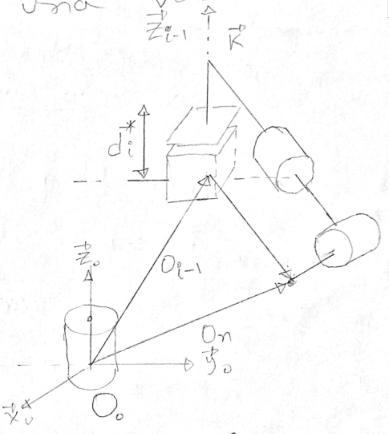
\includegraphics[width=0.3\linewidth]{f2}
\end{figure}
En el dibujo se muestra una articulación prismática que se mueve a lo largo del eje $\vec{z}_{i-1}$ con una velocidad $\frac{d}{dt}d_i$ cuando todas las demás articulaciones se mantienen fijas, resultando en:

$$
\frac{d}{dt} O_n^o(t) = \frac{d}{dt} d_i(t) R_{i-1}^o \vec{k} = \frac{d}{dt}d_i(t) z_{i-1}^0 = J_{\upsilon_i} \dot{d}_i = \upsilon_n^0
$$

por lo tanto $$J_{\upsilon_i}=z_{i-1}^0$$

\begin{figure}[h]
     \centering
    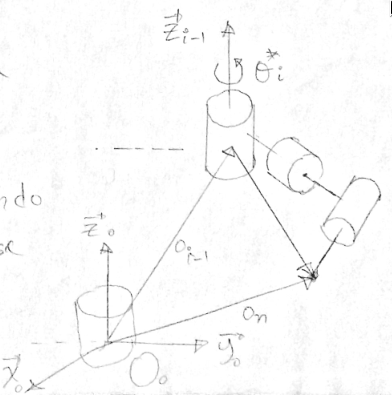
\includegraphics[width=0.3\linewidth]{f3}
\end{figure}
En este dibujo se muestra una articulación revolita $i$, que rota alrededor del eje $z_{i-1}$ con una velocidad angular $\frac{d}{dt}\theta_i z_{i-1}$ , cuando todas las demás articulaciones se mantienen fijas, resultando en:

$$
\frac{d}{dt}O_n^0 = \omega \times r = \begin{bmatrix}
	\dot{\theta}z_{i-1}
\end{bmatrix} \times \begin{bmatrix}
	O_n-O_{i-1}
\end{bmatrix} = J_{\upsilon_i} \dot{\theta_i}
$$

por lo tanto

$$ J_{\upsilon_i} = z_{i-1}^0 \times \begin{bmatrix}
	O_n-O_{i-1}
\end{bmatrix} $$

De lo anterior se tiene que la mitad superior del Jacobiano $J_\upsilon$ esta dada por

$$
J_\upsilon = \begin{bmatrix}
	J_{\upsilon_1} \cdots J_{\upsilon_n}
\end{bmatrix}
$$

donde la i-ésima columna $J_\upsilon$ es

$$
J_{\upsilon_i} = \begin{cases}
	z_{i-1} \times ( O_n-O_{i-1} ) \quad \text{para la articulación revoluta } i \\
	z_{i-1} \quad \text{para la articulación prismática } i
\end{cases}
$$
\newpage
La mitad inferior del Jacobiano esta dada por
$$ J_\omega = \begin{bmatrix}
	J_{\omega_1} \cdots J_{\omega_n}
\end{bmatrix}
$$

donde la i-ésima columna $J_\omega$ es

$$
J_{\omega_i} = \begin{cases}
	z_{i-1} \quad \text{para la articulación revolita } i \\
	0 \quad \text{para la articulación prismática } i
\end{cases}
$$

por lo tanto para un Jacobiano de n-eslabones se tendrá,

$$
J = \begin{bmatrix}
	J_1 & J_2 & \cdots & J_n
\end{bmatrix}
$$
\end{document}
